
Για την υλοποίηση σε Rust είναι αρχικά σημαντικό να ξεκαθαρίσουμε ορισμένα
πράγματα. Ο μεταγλωττιστής της Rust παρέχει στην πραγματικότητα δύο ξεχωριστές
γλώσσες, την ασφαλής (safe) Rust και την μη ασφαλής (unsafe) Rust. Η safe Rust
όπως υπονοεί το όνομα είναι το μέρος της γλώσσας που χρησιμοποιεί στατική ανάλυση
για να αποτρέψει σύνηθες σφάλματα που αφορούν την διαχείριση μνήμης. Η unsafe Rust
ενεργοποιείται με την λέξη κλειδί \verb|unsafe| και επιτρέπει ενέργειες που ενδεχομένως
μπορούν να διακόψουν (halt) την εκτέλεση του προγράμματος, όπως να κάνουμε dereference έναν
σκέτο (raw) δείκτη. Η σύνηθες υλοποίηση της λογικής της Rust που εξηγείτε στα παρακάτω κεφάλαια
διατηρείτε και στις δύο εκδοχές της γλώσσας και όπως θα δούμε μπορούν προφανώς να συνυπάρχουν.

Σε γενικές γραμμές όμως η safe Rust είναι ένα υποσύνολο της unsafe Rust. Μάλιστα διαισθητικά
τουλάχιστον μπορούμε να πούμε πως η safe Rust είναι υποσύνολο της C. Δηλαδή έστω ότι όλα τα πιθανά
προγράμματα εκφράσιμα από μια παραδοσιασκή μηχανή Turing βρίσκονται στο σύνολο $U$, όλα τα πιθανά
προγράμματα εκφράσιμα από το specification της C $C=U$ και όλα τα πιθανά προγράμματα της safe Rust $SR \subseteq C$.
Συνεχίζοντας ισχύει ότι για την unsafe rust $UR=C=U, SR \subseteq UR$. 

Έχωντας πει αυτά γίνεται ξεκάθαρη η πολυπλοκότητα του μεταγλωτιστή. Σε σύγκριση με την C η οποία 
μπορεί να μεταφραστεί σε γλώσσα μηχανής με μόνο ένα ενδιάμεσο στάδιο η Rust χρειάζεται το λιγότερο 3
στην μόνη υλοποίηση που υπάρχει. Σε αυτά τα τέσσερα στάδια, δεν μετριούνται καν οι ενδιάμεσες αναπαραστάσης
του LLVM. Στο σχήμα \ref{fig:rust_ir} η κάθε ενδιάμεση αναπαράσταση μεταλλάζει τον πηγαίο κώδικα σε όλο και
μια πιο απλή γλώσσα που στο τέλος η μηχανή μπορεί να κατανοήσει.

\begin{enumerate}
\item HIR: Είναι ο πηγαίος κώδικας αλλά desugared, δηλαδή οντότητες όπως είναι ο χρόνος
  ζωής μεταβλητών (lifetimes) ή οι τύποι των μεταβλητών εκφράζονται πλέον ρητά. Ένα
  feature σημαντικού ενδιαφέροντος για εμάς που γίνεται desugared σε αυτό το στάδιο είναι τo
  \verb|async|.
\item THIR: Σε αυτήν την αναπαράσταση η απλοποίηση του κώδικα γίνεται πιο εμφανής. Σύνθετη
  τύποι μετατρέπονται σε πιο απλούς (primitives), τα generics μεταφράζονται στις στατικές τους
  μορφές και οι μέθοδοι μετατρέπονται σε συναρτήσεις.
\item MIR: Ο λόγος ύπαρξης του THIR είναι για να γίνεται πιο απλή η μετάφραση σε αυτό το στάδιο.
  Είναι ουσιασικά ένα Control-Flow Graph (CFG) που αναπαριστά την ροή εκτέλεσης του προγράμματος.
  Εδώ γίνεται η στατική ανάλυση απαραίτητη για τον Borrow Checker, τον εγκέφαλο του στατικού ελεγκτή
  της Rust που είναι υπεύθυνος για το specification που πρέπει να ακολουθεί το πρόγραμμα μας. 
\end{enumerate}

Η τελική μετατροπή είναι του LLVM το οποίο είναι ένα third-party framework που χρησιμοποιείτε ως
παγκόσμια γλώσσα μηχανής. Είναι μια υπερβολικά απλή και μινιμαλιστική γλώσσα προγραμματισμού βασισμένη
σε SSA (Static Single Assignment) η οποία μεταφράζεται στις πιο γνωστές αρχιτεκτονικές. Η SSA είναι ιδανική
για να αναπαραστήσει την Rust σε χαμηλότερο επίπεδο κυρίως για την ιδιότητα που έχει όσο αναφορά το code-locality.
Εδώ είναι καλή στιγμή να αναφερθούμε στο specification της Rust, τους κανόνες δηλαδή που ένα πρόγραμμα πρέπει να
ακολουθεί για να γίνει compile.


\begin{enumerate}
  \item Το πρώτο βασικό χαρακτηριστικό της γλώσσας είναι ότι τα σύμβολα είναι σταθερές by default, για να ορίσουμε μεταβλητές
    πρέπει να χρησιμοποιήσουμε την λέξη κλειδί \verb|mut|.    
\begin{lstlisting}[language=Rust]
let x = 5;
x = 6; //Error `x` is not mutable

let mut y = 5;
y = 6; // Valid, since its `mut`
    \end{lstlisting}
  \item Κάθε τιμή στη Rust έχει ένα και μόνο ένα owner. Όταν ο owner της τιμής βγαίνει εκτός
    scope η τιμή αποδεσμεύεται αυτόματα από τη μνήμη.    
\begin{lstlisting}[language=Rust]
fn main() {
    let s = String::from("hello"); 
    //Create inner scope
    {
    let t = s; //`t` now owns `s`
    }
  //Inner scope ends here
  println!("{}", s); // Error: `s` has been consumed/moved
}
\end{lstlisting}
\item Κάθε τιμή μπορεί να έχει άπειρες αμετάβλητες αναφορές $\&Τ$ ή μόνο μια μεταβλητή αναφορά
  $\&mut T$.  
\begin{lstlisting}[language=Rust]
let mut x = 10;
let y = &x; // Immutable reference 
let z = &x; // Valid, can have infinite 
println!("{},{}", y, z);

let w = &mut x; // Error: Cant `&mut T` while `&T` exist
\end{lstlisting}
\end{enumerate}

\begin{figure}[!htb]
    \centering
    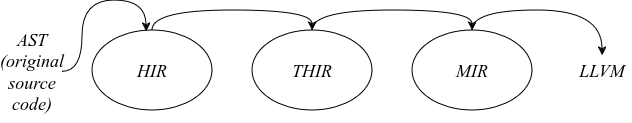
\includegraphics[scale=0.4]{images/rust/rust_irs.png}
    \caption{Rusts Intermediate Representations.}
    \label{fig:rust_ir}
\end{figure}
